\quad U ovom poglavlju zaći ćemo dublje u pojam dobrote i proces selekcije te predložiti nekoliko načina implementacije.

\section{Dobrota}
\quad U 3. poglavlju dotakli smo se pojma dobrote (eng. fitness) te dali kratki i jednostavan opis koji proširujemo ovdje. Dobrota je vrijednost koju koristimo kako bi mogli reći koliko je program dobar u rješavanju danog zadatka i koju koristimo pri međusobnom uspoređivanju različitih programa. Dobrota nema univerzalan način računanja niti univerzalan okvir vrijednosti, ali očekuje se da je program bolji u rješavanju zadatka što je dobrota veća.\par 
U nadziranom učenju naši programi, uz ulazne vrijednosti, dobivaju i očekivane izlazne vrijednosti. Očekivane izlazne vrijednosti služe za uspoređivanje s izlaznim vrijednostima naših programa. Usporedbom dobivamo pogrešku (eng. error) koja nam govori koliko se rezultati naših programa razlikuju od očekivanog izlaza. Pogrešku možemo koristiti kako bi izračunali dobrotu. Način pretvorbe pogreške u dobrotu ostavlja se na izbor osobi koja će implementirati nadzirano učenje, ali ovdje će se predložiti jedna jednostavna operacija. Operacija u pitanju je cjelobrojno dijeljenje broja jedan s pogreškom ($ \frac{1}{error} $). Operacija čini dvije vrijednosti obrnuto proporcionalne i u potpunosti je prihvatljiva opcija.\par 
U podržanom učenju naši programi dobivaju niz ulaznih vrijednosti prema kojima donose "odluke". "Odluke" se mogu ili kazniti ili nagraditi. Kazna i nagrada nisu odmah uočljivi što znači da se program neće ocijeniti pri primitku prve kazne/nagrade. Kazne i nagrade se akumuliraju kroz više "odluka". Primijenimo li primjer igre, naši programi će raditi poteze kroz runde i bit će kažnjeni ili nagrađeni za njih, a na kraju igre dobivaju konačan rezultat koji je procjena koliko su bili uspješni u igri. Ako se radi o zadatku u kojem postoje elementi nasumičnosti bilo bi dobro svaki program nekoliko puta provesti kroz zadatak kako bi se uvjerili da se uvjeti u zadatku nisu poklopili na takav način da program dobije upravo takvu procjenu uspješnosti.\par 
Elitizam je pojam koji smo obradili u 3. poglavlju. U tom poglavlju je pojam dovoljno dobro objašnjen i ovdje ćemo samo napraviti nadogradnju vezanu za CGP. Ako se utvrdi da roditelj i dijete imaju istu dobrotu, dijete će se propagirati u sljedeću generaciju \cite{CGPbook}\cite{CGPpresentation}. Testovima  je dokazano kako je propagacija djeteta u takvim slučajevima izuzetno korisna i efektivna u dobivanju boljih rezultata \cite{CGPbook}.
\par
Dobrota je izuzetno korisna, ali to ne znači da nas ne može zavarati. Problemi koje ćemo navesti nisu toliko vezani uz sam postupak dobivanja dobrote, oni mogu doći iz različitih dijelova sustava koji razvija programe, ali ti problemi utječu na dobrotu koja nas zatim može zavarati i potaknuti na krivi zaključak. Neki od problema koji se mogu vezati uz dobrotu su pretreniranost i nasumičnost zadatka.\par 
Pretreniranost možemo najviše povezati uz nadzirano učenje. Kod pretreniranosti možemo dobiti sjajne rezultate za podatke nad kojima učimo, ali loše rezultate za neviđeni skup podataka. Tu nas dobrota tehnički ne vara, programi sjajno rade na podskupu za učenje, ali programi ne znaju riješiti generalni tip zadatka. To se događa kad se naši programi previše razviju u smjeru rješavanja jako specifičnih zadataka. Posljedica toga je ta da se pretrenirani programi kroz elitizam i selekciju, zbog visoke dobrote, propagiraju dalje i pretreniraju buduće generacije. Problem se može spriječiti boljom generalizacijom skupa za učenje i ograničavanjem broja generacija ili dobrote.
\par
Pod nasumičnost zadatka misli se na problem koji se javlja kod podržanog učenja kad zadatak ima neke elemente nasumičnosti. Kao što je već ranije spomenuto ne znamo kako će se zadatak dalje razvijati i može se dogoditi da u ponavljanjima dođu izrazito teški ili izrazito laki zadaci. Primjerice, može nastupiti slučaj gdje generalno loš program uspješnije rješava svoje zadatka nego što generalno bolji program rješava svoje, a razlog tome je taj da su se nekoliko puta za redom poklopili posebni uvjeti koji su to omogućili. Posljedica ovog problema je propagacija lošijeg programa u sljedeće generacije. Rješenje ovom problemu može biti provođenje programa kroz zadatak više puta ili drukčiji pristup računanju dobrote.

\section{Selekcija}
\quad Selekciju smo spomenuli u 3. poglavlju, a ovdje ćemo ju dodatno obraditi i navesti neke načine implementacije.\par
 Selekcijom odabiremo programe (roditelje) koji će zajedno biti temelji za nove programe koji će se uvesti u sljedećim generacijama. Povlačimo poveznicu s prirodnim svijetom gdje najuspješnije jedinke dobivaju prioritet prilikom parenja i tako osiguravaju prenošenje svojih gena u buduću generaciju. No, kao i u prirodnom svijetu, ne moraju se samo najbolje jedinke pariti i prenositi svoje gene. To pridonosi raznolikosti unutar vrste, a same slabosti u jednoj situaciji mogu postati snage u drugoj. Po uzoru na opisan proces, imamo nekoliko načina na koje možemo implementirati selekciju.
 \par 
 Prvi i najjednostavniji način koji zahtijeva samo sortiranje programa po dobroti bio bi da uzmemo najbolje programe. Naravno varijante ove implementacije su itekako moguće: jedan najbolji program i jedan najlošiji; par programa s početka, par iz sredine i par s kraja sortiranog niza; jedan program s početka i jedan program iz sredine sortiranog niza... Učinkovitost ovakve selekcije upitna je i u ovom radu neistražena tako da se predlažu neki od sljedećih načina implementacije.\par 
 Selekcija proporcionalna dobroti može se zamisliti kao kotač s kazaljkom koji je podijeljen na dijelove. Svaki dio je reprezentacija jednog programa. Veličina dijela proporcionalna je udjelu dobrote programa u zbroju dobrota svih programa. Primjerice, ako zbrojimo dobrote četiri programa i ako je dobrota jednog program pridonijela trećini zbroja, njegov dio na kotaču pokrivat će jednu trećinu kotača.\newline
 \begin{figure}[h]
 	\centering
 	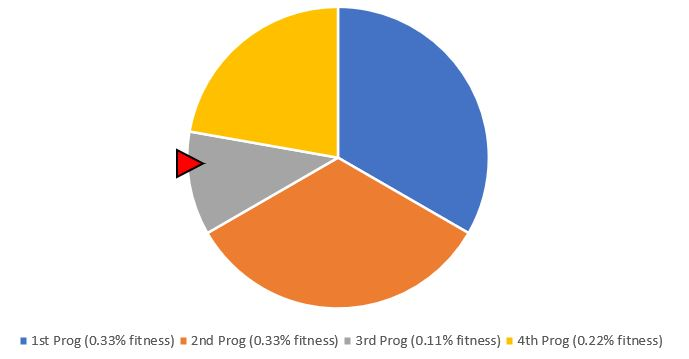
\includegraphics[width=0.9\linewidth]{proporcionalna_selekcija}
 	\caption{Vizualni prikaz selekcije proporcionalne dobroti}
 \end{figure}
 \par 
  Nakon što izračunamo udio svakog programa, nasumično odabiremo programe. Vjerojatnost odabira svakog programa jednaka je njegovom udjelu. Vizualiziramo li taj događaj, zavrtimo kotač i odaberemo program na koji pokazuje kazaljka nakon što se kotač zaustavi. Ovakav oblik implementacije selekcije pokazao se izrazito uspješnim i preporučuje se.
  \par
  Zadnji način implementacije selekcije koji ćemo opisati može biti nadogradnja prethodnom načinu, a naziva se turnir. Nakon što odaberemo nekoliko programa, sasvim nasumice ili po udjelu dobrote, uspoređujemo programe međusobno i najbolji postaju roditelji. Ovaj oblik implementacije daje priliku i slabijim programima jer oni trebaju biti najbolji samo u svojoj skupini, a ne u cijeloj populaciji programa.
  \par
  Selekcija nema nekih osobitih problema koje možemo popraviti. Uvijek postoji mogućnost da ćemo za roditelje odabrati slabije programe ili da će se često odabrati isti programi. Implementacijom gore navedenih strategija pokušava se smanjiti učestalost takvih situacija, a ipak zadržati raznolikost populacije. Ispravna implementacija strategija ključna je za ispravno funkcioniranje selekcije.
  \par
  Ako se tijekom selekcije u CGP-u dogodi slučaj gdje roditelj i dijete imaju istu vrijednost po kojoj se uspoređuju (npr. dobrota), a izbor je između jednog ili drugog, izabrat će se dijete zbog istog razloga koji je naveden za elitizam u prošlom potpoglavlju \cite{CGPbook}\cite{CGPpresentation}. 